% Created 2019-01-27 Sun 16:36
% Intended LaTeX compiler: pdflatex
\documentclass[11pt]{article}
\usepackage[utf8]{inputenc}
\usepackage[T1]{fontenc}
\usepackage{graphicx}
\usepackage{grffile}
\usepackage{longtable}
\usepackage{wrapfig}
\usepackage{rotating}
\usepackage[normalem]{ulem}
\usepackage{amsmath}
\usepackage{textcomp}
\usepackage{amssymb}
\usepackage{capt-of}
\usepackage{hyperref}
\author{Martin Nørskov Jensen}
\date{\today}
\title{}
\hypersetup{
 pdfauthor={Martin Nørskov Jensen},
 pdftitle={},
 pdfkeywords={},
 pdfsubject={},
 pdfcreator={Emacs 26.1 (Org mode 9.1.5)}, 
 pdflang={English}}
\begin{document}

\tableofcontents

\section{Experiments}
\label{sec:org2e7f5df}
\subsection{Relevant facts}
\label{sec:org5d7e7b5}
\begin{itemize}
\item It is assumed that secure facts can be established by the use of senses
\item Most facts can be established using observation
\begin{itemize}
\item Most are irrelevant for science
\end{itemize}
\item Many kinds of processes are at work in the world around us
\begin{itemize}
\item The interact with each other in complicated ways
\item It is necessary to do experiments
\item The discussion take a different perspective when focusing on experiments rather than facts
\end{itemize}
\end{itemize}

\subsection{Producing and updating experimental results}
\label{sec:org54f586c}
\begin{itemize}
\item It is hard and take time to obtain experimental results
\begin{itemize}
\item A significant new experiment takes month or even years to successfully execute
\item It requires practical trial and error and exploitation of the available technology
\item Judgments about the adequacy of experimental results are not straightforward
\item Experiments are only adequate and interpretable
\end{itemize}
\item Experimental results can be faulty if the knowledge informing them is deficient or faulty
\item Experimental results are fallible and can be updated or replaced for straightforward reasons
\begin{itemize}
\item It can be due to advances in technology or advancement in understanding
\end{itemize}
\end{itemize}

\subsection{Transforming the experimental base of science}
\label{sec:orge653a80}
\begin{itemize}
\item The problem with Hertz experiment was not inadequacies in his observation or lack of repeatability
\begin{itemize}
\item The problem was the experimental setup
\end{itemize}
\item Experiments are typically designed to cast light on some signification question
\end{itemize}

\subsection{Experiments as basis for science}
\label{sec:orgbef2ae0}
\begin{itemize}
\item The experimental basis for science is fallible and revisable
\begin{itemize}
\item This poses a threat to the way scientific theories are borne out of experiments
\end{itemize}
\item One cannot make the outcomes conform to our theories
\end{itemize}

\section{Induction}
\label{sec:org75cf0ed}
\subsection{Baby logic}
\label{sec:orga9c2bcb}
\begin{itemize}
\item Logic is concerned with deduction of statements from other statements
\begin{itemize}
\item What follows from what
\item If the premises are true then the conclusion must be true
\item An argument is perfectly valid even though the premises may be wrong
\end{itemize}
\item Logic is not alone a source to new truth
\begin{itemize}
\item Logic can reveal what follows from the statements which we already has
\item Logics great strength is it truth preserving character
\end{itemize}
\end{itemize}

\subsection{Scientific laws from facts?}
\label{sec:org87ba4b7}
\begin{itemize}
\item Scientific knowledge cannot be logically deduced from the facts
\item Arguments who proceed from a finite number of specific facts to a general conclusion is called \textbf{inductive} arguments
\item \textbf{Inductive} arguments are used for general scientific laws need to go beyond what is contained in the premises
\end{itemize}

\subsection{Good inductive argument?}
\label{sec:org927cbc0}
\begin{itemize}
\item If an inductive inference from observable facts to laws is to be justified the following conditions must be satisfied
\begin{enumerate}
\item The number of observations forming a basis for the generalization must be large
\begin{itemize}
\item A large number of independent observations is needed
\item A good argument cannot just jump to conclusions
\end{itemize}
\item The observations must be repeated under a wide variety of conditions
\item No accepted observation statement should conflict with the derived law
\end{enumerate}

\item \textbf{The principle of induction}
\end{itemize}
\begin{center}
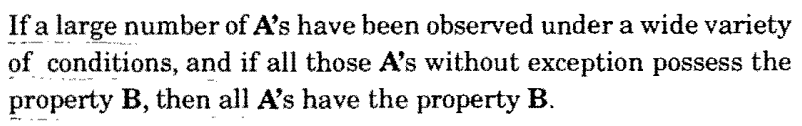
\includegraphics[width=.9\linewidth]{Induction/screenshot_2019-01-27_15-24-02.png}
\end{center}

\begin{itemize}
\item Problems with the conditions
\begin{enumerate}
\item How many is large? and in some scenarios a large number of observations might not be a good idea
\item What counts as a signification variation in circumstances?
\begin{itemize}
\item Prior knowledge is used to look at which factors might have some influence
\item What knowledge can one used and what should one require of that knowledge?
\end{itemize}
\item Little scientific knowledge would survive this demand, that there is no known exceptions
\end{enumerate}
\end{itemize}

\subsection{Problems with inductivism}
\label{sec:org6b7e734}
\begin{itemize}
\item \textbf{Inductivism} is the position according to which scientific knowledge is to derived from using some kind of inductive interference
\begin{itemize}
\item Those who subscribe to that is called \textbf{inductivists}
\end{itemize}
\item Any kind of generalization from facts about the observable world can only yield generalizations about the observable world
\begin{itemize}
\item i.e. inductive reasoning cannot be used for the unobservable world
\end{itemize}
\item Since exact mathematically formulated laws always have some error when measured it is hard to escape the inexactness of the measurements to obtain a law
\item A problem about induction is how can it itself be justified
\begin{itemize}
\item To justify it induction is needed
\end{itemize}
\item Another problem with inductiveness is when one tries to be precise about how probable a law or truth is in the light of the specified evidence 
\begin{itemize}
\item The probability of any general law is zero per standard probability theory
\end{itemize}
\item One cannot provide a rational argument for the rational argument itself without assuming the rational argument
\end{itemize}

\subsection{The appeal of inductivism}
\label{sec:orgb8dcdd5}
\begin{center}
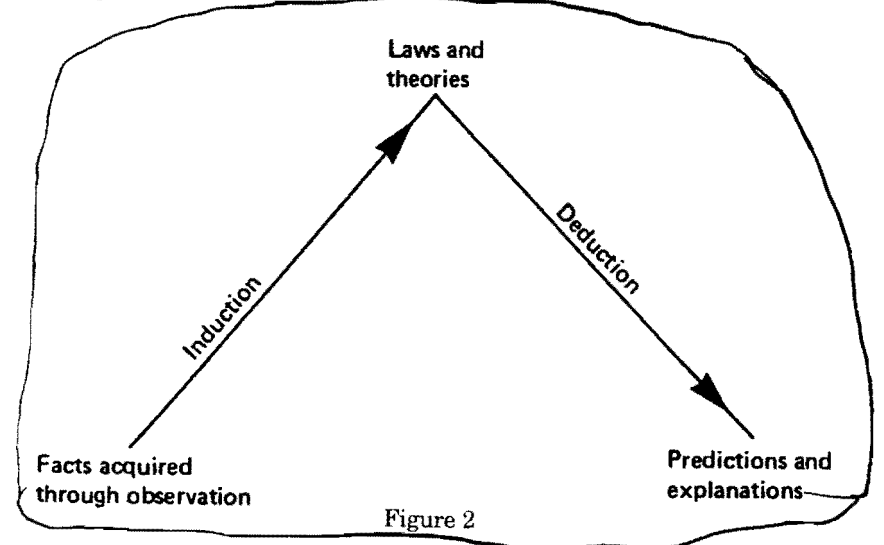
\includegraphics[width=.9\linewidth]{Induction/screenshot_2019-01-27_16-26-08.png}
\end{center} 

\begin{itemize}
\item For the inductivists the source of scientific truth is experience not logic
\item Sets of statements which describe the set-up under investigation is referred to as \textbf{initial conditions}
\item The general form of all scientific explanation and predictions can be summarized as thus
\end{itemize}
\begin{center}
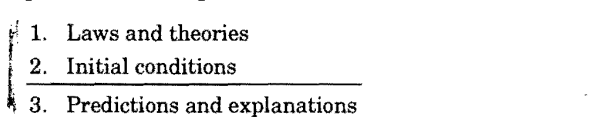
\includegraphics[width=.9\linewidth]{Induction/screenshot_2019-01-27_16-33-38.png}
\end{center} 
\end{document}